\documentclass[11pt]{article}
\usepackage{hyperref}
\usepackage{graphicx}
\usepackage{caption}
\usepackage{geometry}
\usepackage{placeins}
\usepackage{enumitem}
\usepackage{multirow}
\usepackage{float}
\usepackage{wrapfig}
\usepackage{url}
\usepackage{amsmath}
\usepackage{algorithm}
\usepackage{biblatex}
\usepackage{algpseudocode}
\usepackage{tikz}
\usepackage{schemata}
\usepackage{tabularx}
\usepackage{makecell}
\usepackage{pgfplots}
\usepackage[toc,page]{appendix}

\addbibresource{bibliography.bib}


% Set page margins
\geometry{a4paper, margin=1.5cm}

% Set paragraph and spacing
\setlength{\parindent}{0em} % No indentation (annoying)
\setlength{\parskip}{0.5em} % Small space between paragraphs

\graphicspath{{../figures}}

\begin{document}

% TODO: update title
\begin{titlepage}
    \centering
    \vspace*{2cm}
    
    
    {\Huge\bfseries Fuzzy Expert System to Detect \\ Phishing in Websites\par}
    \vspace{1cm}
    % {\large A Comparative Analysis of k-Nearest Neighbors and SVM Classifiers\par}
    
    \vspace{2cm}
    
    {\large
    Dániel MÁCSAI \\ 
    Ismael RUIZ GARCIA \\ 
    Mauro VÁZQUEZ CHAS
    \par}
    
    \vspace{2cm}
    
    {\large
    \textbf{Master in Artificial Intelligence}
    \par}
    
    
\includegraphics[width=0.4\textwidth]{Logo_URV.png}\par\vspace{1cm}

    \vspace{1cm}

    {\large
    Planning and Approximate Reasoning\\
    Delivery 3
    \par}
    
    \vspace{1cm}
    
    {\large\bfseries 15th December 2024\par}
    
\end{titlepage}


% Index
\newpage

\tableofcontents
\newpage

%---------------------------------------------------------------------------------------------------------------------------------
\section{Introduction}
For this work, we 
% TODO  write introduction

\section{Task 1}
To design the fuzzy expert system to detect phishing websites, we consulted \cite{main_paper}. In this paper, they list 87 posible features (boolean, floats and integers) that could matter in the detection of phishing websites. The proposed features are divided into three categories: URL-based features, content features and external features. From this proposed variables, we selected 5 features that we consider relevant for the detection of phishing websites.

\subsection{Chosen Features}


\subsubsection{URL-based features:}
\textbf{Phish Hints} 
\begin{itemize}
    \item \textbf{Description:} Number of words in the URL that are typical of phishing websites
    \item \textbf{Integer}. Number 51 in the paper
\end{itemize}

\begin{figure}[H]
    \centering
    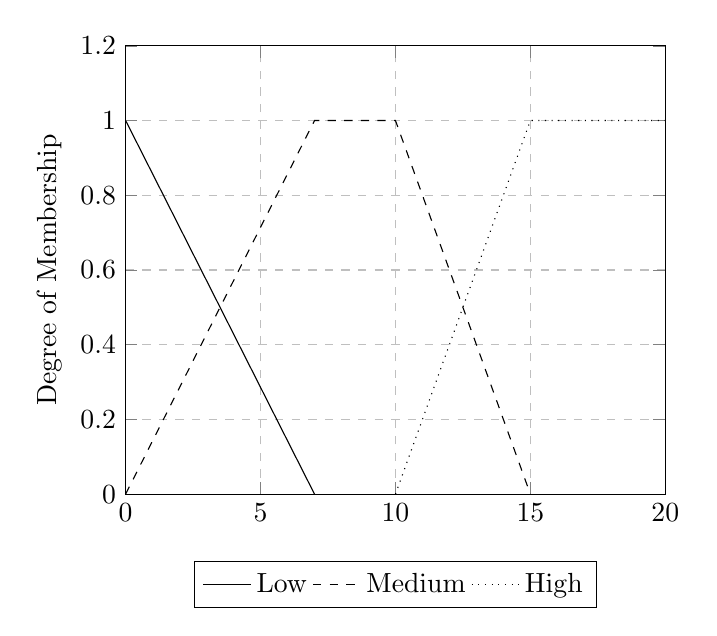
\begin{tikzpicture}
        \begin{axis}[
            ylabel={Degree of Membership},
            ymin=0, ymax=1.2,
            xmin=0, xmax=20,
            legend style={at={(0.5,-0.15)},anchor=north,legend columns=-1},
            ymajorgrids=true,
            xmajorgrids=true,
            grid style=dashed
        ]
        
        % Membership function for "Low"
        \addplot[solid, black] coordinates {(0,1) (0,1) (7,0)};
        \addlegendentry{Low}
        
        % Membership function for "Medium"
        \addplot[dashed, black] coordinates {(0,0) (7,1) (10,1) (15,0)};
        \addlegendentry{Medium}
        
        % Membership function for "High"
        \addplot[dotted, black] coordinates {(10,0) (15,1) (20,1)};
        \addlegendentry{High}
        
        \end{axis}
    \end{tikzpicture}
    \caption{Membership Function Phish Hints}
\end{figure}




\textbf{Domain Age} 
\begin{itemize}
    \item \textbf{Description:} Age of the page in months
    \item \textbf{Integer}. Number 83 in the paper
\end{itemize}

\begin{figure}[H]
    \centering
    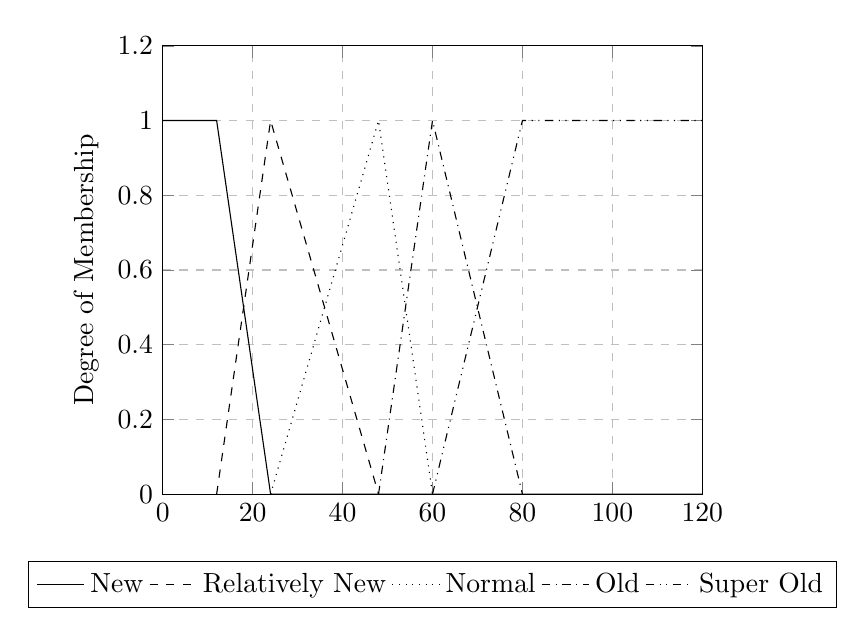
\begin{tikzpicture}
        \begin{axis}[
            ylabel={Degree of Membership},
            ymin=0, ymax=1.2,
            xmin=0, xmax=120,
            legend style={at={(0.5,-0.15)},anchor=north,legend columns=-1},
            ymajorgrids=true,
            xmajorgrids=true,
            grid style=dashed
        ]
        
        % Membership function for "New"
        \addplot[solid, black] coordinates {(0,1) (12,1) (24,0) (120,0)};
        \addlegendentry{New}
        
        % Membership function for "Relatively New"
        \addplot[dashed, black] coordinates {(12,0) (24,1) (48,0)};
        \addlegendentry{Relatively New}
        
        % Membership function for "Normal"
        \addplot[dotted, black] coordinates {(24,0) (48,1) (60,0)};
        \addlegendentry{Normal}
        
        % Membership function for "Old"
        \addplot[dash dot, black] coordinates {(48,0) (60,1) (80,0)};
        \addlegendentry{Old}
        
        % Membership function for "Super Old"
        \addplot[dash dot dot, black] coordinates {(60,0) (80,1) (120,1)};
        \addlegendentry{Super Old}
        
        \end{axis}
    \end{tikzpicture}
    \caption{Membership Function Domain Age (in months)}
\end{figure}



\subsubsection{Content features:}
\textbf{Ratio External Hyperlinks} 
\begin{itemize}
    \item \textbf{Description:} The number of external hyperlinks in a web page divided by the total number of hyperlinks
    \item \textbf{Float}. Number 59 in the paper
\end{itemize}

\begin{figure}[H]
    \centering
    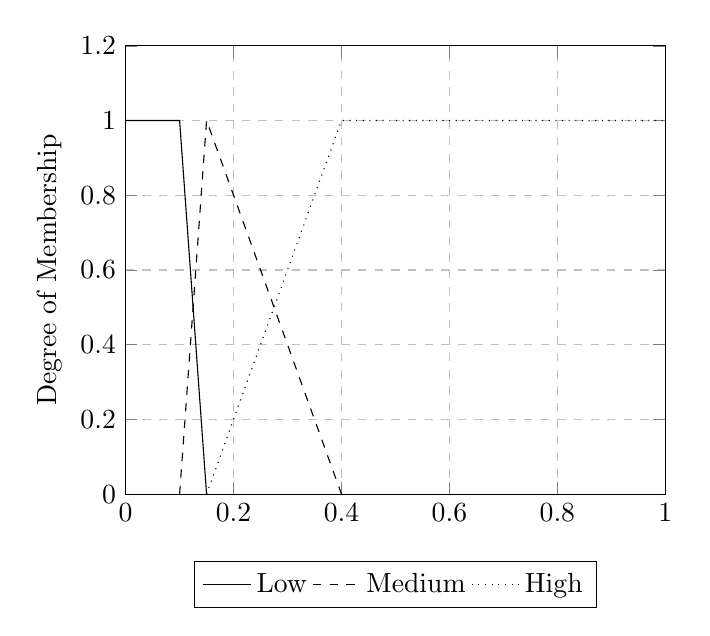
\begin{tikzpicture}
        \begin{axis}[
            ylabel={Degree of Membership},
            ymin=0, ymax=1.2,
            xmin=0, xmax=1,
            legend style={at={(0.5,-0.15)},anchor=north,legend columns=-1},
            ymajorgrids=true,
            xmajorgrids=true,
            grid style=dashed
        ]
        
        % Membership function for "Low"
        \addplot[solid, black] coordinates {(0,1) (0.1,1) (0.15,0)};
        \addlegendentry{Low}
        
        % Membership function for "Medium"
        \addplot[dashed, black] coordinates {(0.1,0) (0.15,1) (0.4,0)};
        \addlegendentry{Medium}
        
        % Membership function for "High"
        \addplot[dotted, black] coordinates {(0.15,0) (0.4,1) (1,1)};
        \addlegendentry{High}
        
        \end{axis}
    \end{tikzpicture}
    \caption{Membership Function Ratio External}
\end{figure}







\subsubsection{External features:}
\textbf{Google Index} 
\begin{itemize}
    \item \textbf{Description:} Whether a page is indexed in Google
    \item \textbf{Boolean}. Number 86 in the paper
\end{itemize}

\begin{figure}[H]
    \centering
    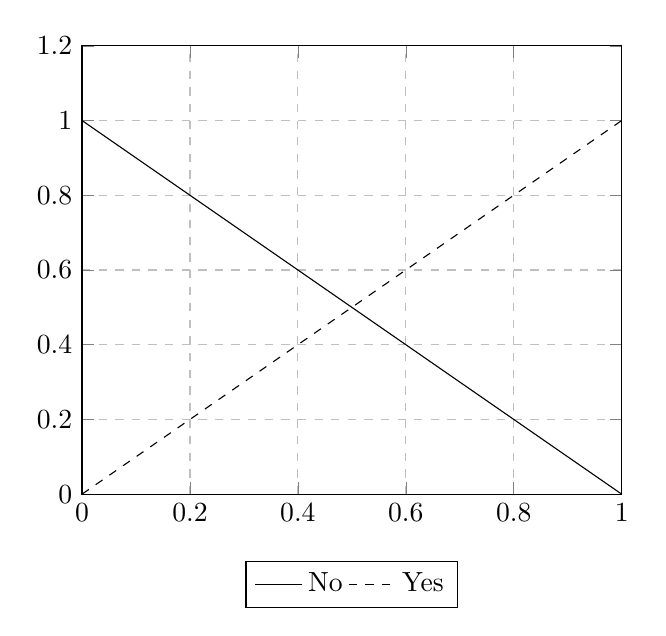
\begin{tikzpicture}
        \begin{axis}[
            ymin=0, ymax=1.2,
            xmin=0, xmax=1,
            legend style={at={(0.5,-0.15)},anchor=north,legend columns=-1},
            ymajorgrids=true,
            xmajorgrids=true,
            grid style=dashed
        ]
        
        % Membership function for "No"
        \addplot[solid, black] coordinates {(0,1) (1,0)};
        \addlegendentry{No}
        
        % Membership function for "Yes"
        \addplot[dashed, black] coordinates {(0,0) (1,1)};
        \addlegendentry{Yes}
        
        \end{axis}
    \end{tikzpicture}
    \caption{Membership Function Google Index}
\end{figure}





\textbf{Page Rank} 
\begin{itemize}
    \item \textbf{Description:} In the end, we chose Google PageRank which follows the same mantra
    \item \textbf{Integer}. Number 87 in the paper
\end{itemize}

\begin{figure}[H]
    \centering
    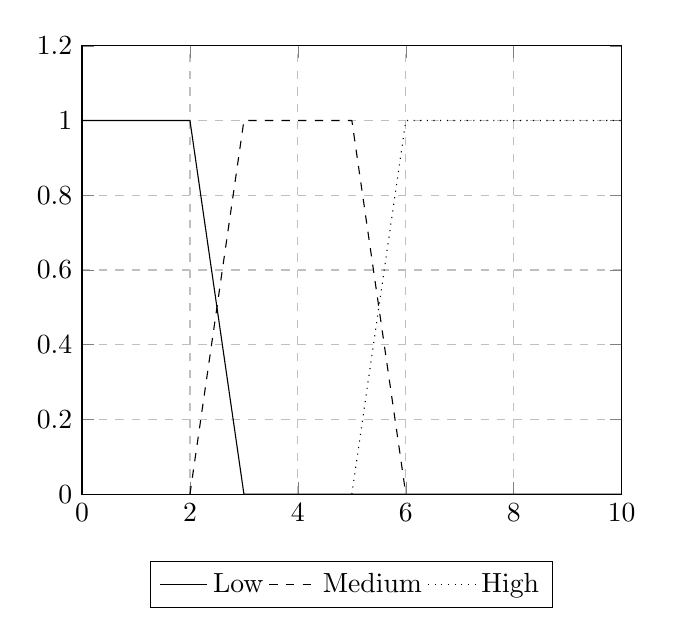
\begin{tikzpicture}
        \begin{axis}[
            ymin=0, ymax=1.2,
            xmin=0, xmax=10,
            legend style={at={(0.5,-0.15)},anchor=north,legend columns=-1},
            ymajorgrids=true,
            xmajorgrids=true,
            grid style=dashed
        ]
        
        % Membership function for "Low"
        \addplot[solid, black] coordinates {(0,1) (2,1) (3,0) (10,0)};
        \addlegendentry{Low}
        
        % Membership function for "Medium"
        \addplot[dashed, black] coordinates {(2,0) (3,1) (5,1) (6,0)};
        \addlegendentry{Medium}
        
        % Membership function for "High"
        \addplot[dotted, black] coordinates {(5,0) (6,1) (10,1)};
        \addlegendentry{High}
        
        \end{axis}
    \end{tikzpicture}
    \caption{Membership Function Google Page Rank}
\end{figure}



\section{Output Variable}
Our output variable will be the phishing risk, where we will consider 5 different fuzzy sets, see \ref{output_variable}.

\begin{figure}[H]
    \centering
    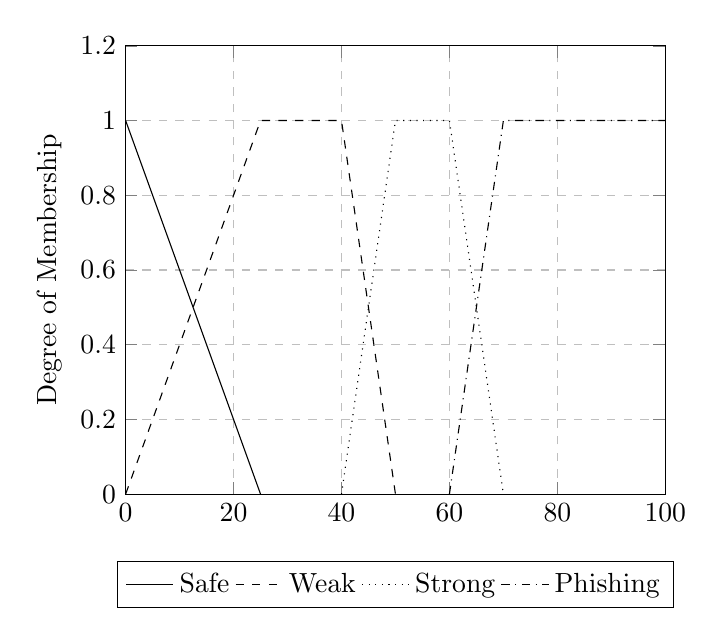
\begin{tikzpicture}
        \begin{axis}[
            ylabel={Degree of Membership},
            ymin=0, ymax=1.2,
            xmin=0, xmax=100,
            legend style={at={(0.5,-0.15)},anchor=north,legend columns=-1},
            ymajorgrids=true,
            xmajorgrids=true,
            grid style=dashed
        ]
        
        % Membership function for "Safe"
        \addplot[solid, black] coordinates {(0,1) (0,1) (25,0)};
        \addlegendentry{Safe}
        
        % Membership function for "Weak"
        \addplot[dashed, black] coordinates {(0,0) (25,1) (40,1) (50,0)};
        \addlegendentry{Weak}
        
        % Membership function for "Strong"
        \addplot[dotted, black] coordinates {(40,0) (50,1) (60,1) (70,0)};
        \addlegendentry{Strong}
        
        % Membership function for "Phishing"
        \addplot[dash dot, black] coordinates {(60,0) (70,1) (100,1)};
        \addlegendentry{Phishing}
        
        \end{axis}
    \end{tikzpicture}
    \caption{Membership Function Phishing Risk (Output Variable)}
    \label{output_variable}
\end{figure}

\section{Rules}

\section{Implementation}
- Mamdami system (min as t-norm and max as t-conorm)
- Defuzzification Method: Center of Area
- Validate the system using the 3D plot of the rules. ??????????? WTF %TODO

\section{Testing}
- 4 Test case that represent different situation (some must activate more than one lable)
- Report the results of each testing case with 
screenshots  and  explanations  that  justify the output  obtained  (i.e.  showing  the  activations of  
rules)

\section{Complex Fuzzy Expert System}
Design (just graphically, no implementation) a more complete fuzzy expert system that 
includes more features about the websites. Show in a figure the inputs, outputs, and rule blocks 
that you propose for such expert system. No specific definition of variables nor rules is required. 

- We can use a hirarchical rule system

% Bibliography
\newpage
\printbibliography


\end{document}